\section{pca\_visual\_extract} \label{sec-pcavisual}

\subsection{General}

The PCA visual extract tool allows you to visualize a sequence dataset,
that has been transformed to a k-mer reprenstation on which PCA was performed
on, and select sequences using a graphical user interface. In order to
calculate the necessary representations the reader might look at the tools
\emph{fasta2kmer} and \emph{kmer2pca} highlighted in sections
\ref{sec-fasta2kmer} and \ref{sec-kmer2pca} respectively.

\subsection{Usage}
The Interface for the \emph{pca\_visual\_extract} tool can be brought
up by calling:
\lstset{language=bash,
  caption={Calling the \emph{pca\_visual\_extract} tool},
  label=lst-pcavisualex-call}
\begin{lstlisting}
pca_visual_extract [fasta] [pca] [dimensions] [first-dim] [second-dim] \
  [out-fasta]
\end{lstlisting}
with the arguments being:
\begin{enumerate}
  \item \emph{fasta} A FASTA file that has been processed by the
    \emph{fasta2kmer} and \emph{kmer2pca} tools (c.f. sections
    \ref{sec-fasta2kmer} and \ref{sec-kmer2pca}) to create a
    representation of the dataset in a PCA subspace.
  \item \emph{pca} The projections onto the principal components as
    generated by \emph{kmer2pca}.
  \item \emph{dimensions} The number of principal componants the
    sequences have been projected onto. The number of dimensions of
    the PCA subspace.
  \item \emph{first-dim} The first principal component to visualize.
  \item \emph{second-dim} The second principal component to visualize.
  \item \emph{out-fasta} A FASTA file where the selected sequences
    will be written to. 
\end{enumerate}
Here \emph{first-dim} and \emph{second-dim} allow you to choose an
arbitrary plane spun by two principal components to select your
sequences in a visual manner. Once the call to the program was issued
on the shall and all the arguments are coherent a graphical user
interface as shown in figure \ref{fig-pcavisual} is presented on the
screen. On the top of figure \ref{fig-pcavisual} you see a
window in which you can draw a rectangle using your mourse
curser. The terminal as shown below than shows you how many
sequences you have selected. Once you are fine with your
selection you might hit the Enter key in order to write out your
selection to a FASTA file.
\begin{figure}
  \begin{center}
    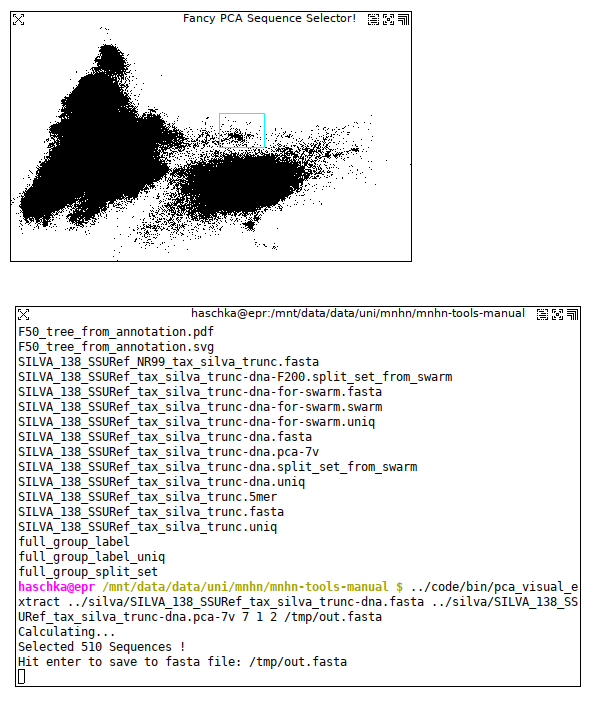
\includegraphics{pca-sequence-selector.png}
    \caption{The color inverted interface of the
      \emph{pca\_visual\_sequence\_selector}.}
    \label{fig-pcavisual}
  \end{center}
\end{figure}

\subsection{Example}
\lstset{language=bash,
  caption={Example of the \emph{pca\_visual\_extract} tool},
  label=lst-pcavisualex-example}
\begin{lstlisting}
pca_visual_extract test.fast test.pca 7 2 3 /tmp/out.fasta
\end{lstlisting}
Will bring up an interface such as the one shown in figure
\ref{fig-pcavisual}, representing the sequences in \emph{test.fasta} in
their 7 dimensional PCA subspace as stored in \emph{test.pca}. A two
dimensional image representing the second and third principal
component is drawn. Using the mouse one can draw a rectangle selecting
sequences. Once the right sequences are selected hitting the Enter key
will store them to \emph{/tmp/out.fasta}.

\subsection{Implementation}
The tool is implemented in \emph{pca\_visual\_extract.c} and makes use
of the Simple Direct Layer 2 (SDL2) library for its drawing routines
and portability across systems.

